\chapter{Introduction}
\label{ch:intro}

In the last years, the volume of semantic data available, in particular in RDF format, has dramatically
increased. Initiatives like the W3C Semantic Web and the Linked Open Data  have great contribution in such
development. The first provides a common standard that allows data to be shared and reused across different
applications, and the latter enables linkages between different datasets that are not originally interconnected.
Moreover, advances in information extraction have made a strong contribution by crawling multiple non-structured
resources in the Web in order to extract RDF facts.

While it provides useful date, information extraction is still limited, since many of its sources might contain
contradictory or uncertain information. Therefore, many of the extracted datasets suffer from incompleteness, noise and
uncertainty. The first means that there are facts which are not existent in the dataset,  and the second means that
the dataset might contain facts which are not true, and the latter one means that the truthfulness of the facts is not
certain. These problems make it much more challenging to automatically learn rules from the data.

%Moreover, for noisy and incomplete knowledge bases, the automatic (i.e., unsupervised) selection of positive and
%negative training examples needed for learning new rules poses a major challenge to the adoption of these techniques.

In order to reduce such problems, one can apply a set of inference rules that describes the knowledge base domain.
They make it possible to resolve contradictions as well as strengthen or weaken the confidence values of facts. It is
also possible to derive new facts that are originally not existent due to incompleteness. Such inference rules can
either represent consistency constraints (\emph{hard rules}), or rules that hold for most but all cases in real
world (\emph{soft rules}).

In this thesis, we consider only inference rules that can be represented as Datalog clauses. In a nutshell,
a Datalog clause is a logic program inference clause composed a list of body predicates as the premise, and a
head predicate as conclusion, where each predicate is a tuple with variables or constants as arguments. A Datalog clause
is safe if all the variables present in the head are also present in the body, moreover, negated predicates are allowed
in the body as long as every variable present in a negated predicate is also present in a non-negated predicate.

An example of safe Datalog rule, which states that married people usually live in the same place as their spouse,
could be written as follows:

\begin{center}
  $\underbrace{livesIn(X,Y)}_{head}$ :- $\underbrace{marriedTo(X,Z),livesIn(Z,Y)}_{body}$
\end{center}

If we have an incomplete knowledge base, which lacks information about where \emph{Michelle Obama} lives, but
contains the facts $marriedTo(michelleObama,barackObama)$ and $livesIn(barackObama,washingtonDC)$, we could apply the
aforementioned rule to derive the fact $livesIn(michelleObama, washingtonDC)$. 


%http://people.csail.mit.edu/kersting/profile/PROFILE_ilp.html

Such rules are rarely known beforehand, but the data itself can be used to mine them using Inductive Logic
Programming (ILP). ILP is a well-established framework for inductively learning relational descriptions (in the form
of logic programs) from examples and background knowledge. Given a logical database of facts, an ILP system will
generate hypotheses in a pre-determined order and test them against the examples. However, in a large knowledge base,
ILP becomes too expensive, since the search space grows combinatorially with the knowledge base size, and the larger the
number of examples, the more expensive it is to test each hypothesis.

Although it is very expensive to learn rules with constants, such kind of rules can be extremely interesting as they
can express particular characteristics of specific groups. For example, the rule $speaks(X,Y)$ :- $livesIn(X,Z)$ is not
very meaningful. It simply tells that people who live somewhere also speak some language. Nevertheless, if we
consider setting constant values for $Y$ and $Z$, we can learn much more valuable rules such as
$speaks(X,english)$ :- $livesIn(X,australia)$ or $speaks(X,spanish)$ :- $livesIn(X,mexico)$.

The problem is that for learning such examples, it would be necessary to test rules with all combinations of
countries and languages, which surely can lead to a very expensive process when applied on large databases. Given the
huge size of the search space and the great interestingness of this kind of rules with constants, it is appropriate to
reduce the search space by pruning constants or combinations of constants which are not correlated to the
hypothesis.

The literal $bornInMonth(X,april)$, for example, does not have any correlation  to $speaks(X,spanish )$ :-
$livesIn(X,mexico)$ or $speaks(X,english)$ :- $livesIn(X,australia)$. So if we add such literal to the body of any of
these clauses, it would most likely not cause any change to the confidence,  but certainly a reduction in the support,
therefore it is not interesting to test such hypotheses with the addition of uncorrelated literal.

%This will give as output a set of rules which should satisfy a minimum support and confidence.

\section{Motivation}

For numerical properties, it might be also relevant to search for interesting constants. Nevertheless, for very large
or infinite numerical domains, such as the real numbers for instance, setting a numerical constant as an individual
value will very likely have a single entity associated. In such a case, it would be equivalent to simply
specifying a constant for this given entity without the necessity of adding the numerical property

For example, it is extremely unlikely that a country has the exact same GDP or population as any other country. If we
have the following rule with the attribute $hasPopulation$, whose domain is the positive integer numbers
$\mathbb{N}^+$:

\begin{center}
 $speaks(X,portuguese)$ :- $livesIn(X,Z),hasPopulation(Z,193946886)$
\end{center}

As Brazil is the only country with a population of $193,946,886$ inhabitants, the rule above would be equivalent to:

\begin{center}
 $speaks(X,portuguese)$ :- $livesIn(X,brazil)$
\end{center}

Clearly, if we have to choose between one of the two rules, the latter one would be preferred, since is shorter and
specifies the country in a clearer manner. Moreover, by setting numerical constants punctually, we would end up having a
huge number of different constants to test in the hypothesis and most of them would be most likely discarded because of
low support.

Therefore, it is interesting to consider numerical intervals instead of points, and discretize the attribute's domain
into buckets, and subsequently check if any of them present different confidence in comparison to its
correspondent numerical constant-free rule (which we will call ``base-rule'').

For example if we test the hypothesis and we find support=100 and confidence=0.4:

\begin{center}
 $isMarriedTo(X,Y)$ :- $hasAge(X,Z)$ 
\end{center}

and then split the domain of $Z$ into three buckets:

\begin{itemize}
 \item $ b_1: Z\in[0,20]$
 \item $ b_2: Z\in(20,40]$
 \item $ b_3: Z\in(40,\infty]$
\end{itemize}

We can generate three refined-rules by restricting the base-rule's domain from variable $Z$:

\begin{itemize}

 \item $isMarriedTo(X,Y)$ :- $hasAge(X,Z), z\in[0,20]$	
    %\newline support=4, confidence=0.1
    \newline support=40, confidence=0.1
 \item $isMarriedTo(X,Y)$ :- $hasAge(X,Z), z\in(20,40]$	
    %\newline support=20, confidence=0.5
    \newline support=40, confidence=0.5
 \item $isMarriedTo(X,Y)$ :- $hasAge(X,Z), z\in(40,\infty]$
    %\newline support=16, confidence=0.8
    \newline support=20, confidence=0.8

\end{itemize}

For the buckets $b_2$ and $b_3$, we have a significant confidence gain in comparison to the base-rule.
Furthermore, adding a relation to the body might produce totally different support and confidence distributions along
the buckets. For example, if we add the relation $hasChild(X,A)$, we could obtain other interesting rules:

Base-rule:
\begin{itemize}
 \item $sMarriedTo(X,Y)$ :- $hasAge(X,Z),hasChild(X,A)$	
    \newline support=42, confidence=0.76
\end{itemize}

Refined-rules:
\begin{itemize}
 \item $isMarriedTo(X,Y)$ :- $hasAge(X,Z),hasChild(x,a), Z\in[0,20]$	
    \newline support=2, confidence=0.5
 \item $isMarriedTo(X,Y)$ :- $hasAge(X,Z),hasChild(x,a), Z\in(20,40]$	
    \newline support=20, confidence=0.75
 \item $isMarriedTo(X,Y)$ :- $hasAge(X,Z),hasChild(x,a), Z\in(40,\infty]$	
    \newline support=20, confidence=0.8
\end{itemize}

\begin{figure}
\label{fig:addingHasChildExample}

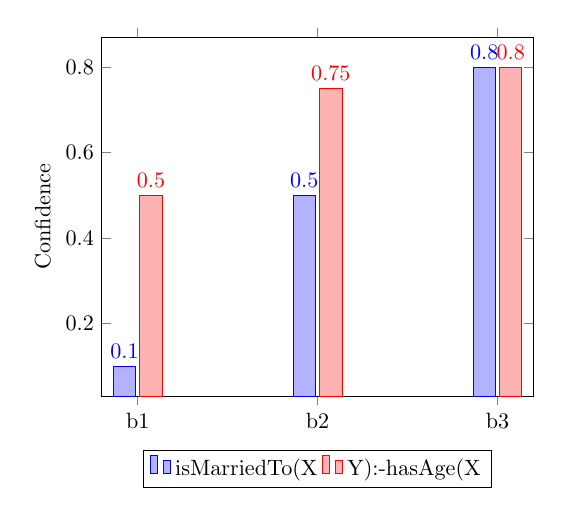
\begin{tikzpicture}[scale=0.8]
\begin{axis}[
    ybar,
    enlargelimits=0.10,
    legend style={at={(0.5,-0.15)},
      anchor=north,legend columns=-1},
    ylabel={Confidence},
    symbolic x coords={b1,b2,b3},
    xtick=data,
    nodes near coords,
    nodes near coords align={vertical},
    ]
\addplot coordinates {(b1,0.1) (b2,0.5) (b3,0.8)};
\addplot coordinates {(b1,0.5) (b2,0.75) (b3,0.8)};
\legend{isMarriedTo(X,Y):-hasAge(X,Z) , isMarriedTo(X,Y):-hasAge(X,Z)hasChild(X,A)}
\end{axis}
\end{tikzpicture}
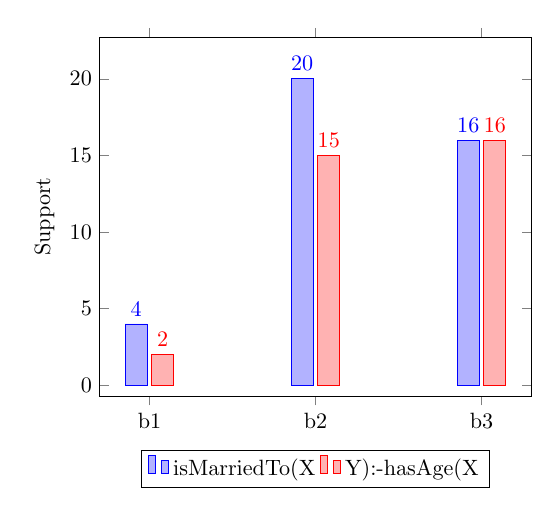
\begin{tikzpicture}[scale=0.8]
\begin{axis}[
    ybar,
    enlargelimits=0.15,
    legend style={at={(0.5,-0.15)},
      anchor=north,legend columns=-1},
    ylabel={Support},
    symbolic x coords={b1,b2,b3},
    xtick=data,
    nodes near coords,
    nodes near coords align={vertical},
    ]
\addplot coordinates {(b1,4) (b2,20) (b3,16)};
\addplot coordinates {(b1, 2) (b2,15) (b3,16)};
\legend{isMarriedTo(X,Y):-hasAge(X,Z), isMarriedTo(X,Y):-hasAge(X,Z)hasChild(X,A)}
\end{axis}
\end{tikzpicture}
\end{figure}

Adding a certain predicate to the rule might not bring any gain or even loss in confidence to the base-rule, but when
bucketing per age, it might present a different confidence distribution, with potential confidence gain for specific
intervals.

On the other hand, adding a predicate with no correlation to the rule might not generate any gain. Hence, it is
necessary to carefully choose the relations and eventual constants, discarding those with no correlation to the rule.  

\section{Contributions}
In this thesis, we propose a preprocessing step, in which for each numerical property we want to investigate,
we build a graph we call correlation lattice. Each graph has a numerical property as its root, where we first
query the examples distribution along the numerical attribute, and build a histogram by discretizing them into $k$
buckets. Subsequently, we  pick a set of $c$ categorical properties that can be joined with the root, extract the
frequencies histogram and analyze how the distribution of the resulting sub-population is affected. Afterwards, we try
to combine the categories and check whether they still produce interesting sub-populations, creating a lattice
structure which resembles that of frequent itemset mining.

We compare the distributions obtained from the frequencies histograms using information theoretical measures,
such as Kullback-Leibler divergence, as well as independence checks, such as Pearson's Chi-squared, in order to
measure the interestingness of adding literals to clauses.

Moreover, we discuss the pruning opportunities and evaluate different heuristics, interestingness measures, and
their efficiency in finding rules with numerical intervals. 

\begin{comment}
In a clause containing a numerical attribute in the body, we can obtain a support and confidence as well as support
value for each of the buckets. Therewith, we can search the most interesting intervals that satisfies the support and
confidence thresholds
\end{comment}

With the information about different distributions contained in the generated lattice, once we add one of the
root properties during the core ILP algorithm, we can try to predict whether the rule has interesting intervals for the
given numerical attribute, and prevent expensive queries from being executed. Furthermore, for a given clause, we
can also suggest the most interesting literals to be added to the body in the subsequent refinement step.

In summary, we present in this thesis three main contributions:

\begin{itemize}

 \item An efficient way of learning rules with combinations of numerical and categorical attributes.
 \item An evaluation of different interestingness measures, which indicate the potential of finding of finding
interesting numerical intervals
 \item The correlation lattice, its properties and how to efficiently build it with pruning techniques and heuristics.
 \item An extension to ILP using the correlation lattices information as heuristics to reduce the search space.
 \item Experiments on Linked Open Data datasets.
\end{itemize}


%\section{Outline}

%The rest of this thesis is structured as follows. In Chapter~\ref{sec:rw-intro} we briefly present ..

\begin{comment}
 The remainder of this thesis is structured as follows. In
Chapter~\ref{ch:technical_background}, we provide technical background on
MapReduce and BigTable. In Chapter~\ref{ch:related_work}, we present a
summary of previous work in the areas of duplicate and near-duplicate detection,
information retrieval on web archives, and MapReduce applications in graph
processing. Following that, we state our problem and describe solutions in
Chapter~\ref{ch:redundancy_control}. In Chapter~\ref{ch:mapreduce_impl}, we
describe an implementation of our solution using the MapReduce framework. In
Chapter~\ref{ch:experiments}, we present our experimental results. We conclude
this thesis and outline directions of future research in Chapter~\ref{ch:future_work}.
\end{comment}
